% Self-contained manuscript. References are embedded; no .bib file is needed.
% Build: pdflatex ncm_systems_paper.tex (twice), or tectonic ncm_systems_paper.tex
% This article describes the tpu-ncm 0.1.0 implementation snapshot.
\documentclass[11pt,a4paper]{article}
\usepackage[T1]{fontenc}
\usepackage[utf8]{inputenc}
\usepackage{lmodern}
\usepackage[margin=25mm]{geometry}
\usepackage{amsmath,amssymb}
\usepackage{booktabs,tabularx,array}
\usepackage{microtype}
\usepackage{xcolor}
\usepackage{enumitem}
\usepackage{listings}
\usepackage{tikz}
\usetikzlibrary{arrows.meta,positioning,fit}
\usepackage[numbers,sort&compress]{natbib}
\usepackage{hyperref}
\hypersetup{colorlinks=true,linkcolor=blue!45!black,citecolor=blue!45!black,
  urlcolor=blue!45!black,pdftitle={A Functional JAX/Flax Implementation of Next-Concept Modeling for TPU-Oriented Execution},
  pdfauthor={Fabian Balensiefer}}
\urlstyle{same}
\setlength{\emergencystretch}{2em}
\setlist{nosep,leftmargin=*}
\lstset{basicstyle=\ttfamily\footnotesize,breaklines=true,
  columns=fullflexible,keepspaces=true,frame=single,rulecolor=\color{black!20},
  backgroundcolor=\color{black!2},showstringspaces=false}
\newcommand{\sg}{\operatorname{sg}}
\newcommand{\Ind}{\mathbb{1}}
\newcommand{\R}{\mathbb{R}}
\newcommand{\code}[1]{\texttt{\detokenize{#1}}}
\newcommand{\safe}[1]{\max\!\left(1,#1\right)}
\newcolumntype{Y}{>{\raggedright\arraybackslash}X}

\title{A Functional JAX/Flax Implementation of\protect\\
Next-Concept Modeling for TPU-Oriented Execution}
\author{Fabian Balensiefer}
\date{November 11, 2026}

\begin{document}
\maketitle

\begin{abstract}
Next-Concept Modeling (NCM) represents a sequence through multiscale discrete
codes and generates each level in parallel, conditioned on earlier levels.
This paper documents an independent, unnamed implementation of that approach
using JAX and Flax, with a focus on explicit state and accelerator execution
contracts. The repository implements a text encoder and decoder, scanned
residual vector quantization, functional exponential-moving-average codebooks,
a parameter-shared level-wise Transformer, and explicit data/model sharding.
Additional implementation objectives include differentiable marginal entropy,
optional aligned concept consistency, runtime codebook freezing, and fixed-shape
byte fallback routing. We formalize the masking and conditioning paths, identify
the gradient boundaries in the joint training step, and analyze the costs of
padding all hierarchy levels to a common length. Validation comprises eleven
passing CPU tests, including a four-device virtual CPU comparison of a
\(2\times2\) data/model mesh with an unsharded reference, plus a three-step
synthetic training example. These are software correctness checks; they do not
establish language-model quality, compression gains, TPU throughput, or
multi-host scalability. We give a controlled evaluation plan and specify the
remaining data, checkpointing, and Rust tooling work needed for a complete
research system.
\end{abstract}

\noindent\textbf{Keywords:} next-concept modeling; residual vector quantization;
JAX; Flax; TPU; SPMD; hierarchical generation.

\section{Introduction}
Hierarchical discrete representations provide an interface between a learned
codec and a generative prior. Next-Concept Modeling (NCM), introduced by
\citet{kumbong2026ncm}, combines multiscale residual quantization with
coarse-to-fine text generation. This paper concerns an independent systems
implementation of that idea rather than a new claim of inventing NCM. The
project model has no separate name; \code{tpu-ncm} is a software package identifier.

Translating a generative design into a compiled distributed program requires
decisions that are not captured by its high-level factorization. A quantizer
must exclude padding from sufficient statistics, preserve codebook consistency
across data shards, and distinguish trainable parameters from moving-average
state. A level-wise generator must condition on the cumulative representation
available before predicting its current level. Shape-stable control flow must
also preserve the semantics of codebook freezing and quantizer dropout.

The implementation uses JAX transformations~\citep{jax} and the Flax Linen
module API~\citep{flax,flaxscan}. XLA provides the compilation layer~\citep{xla}.
Rust is reserved for a proposed surrounding data and orchestration layer; no
Rust component is present in the evaluated snapshot. The implementation is
available in the public project repository, version 0.1.0, with this manuscript
describing the November 11, 2026 snapshot~\citep{localrepo}. Source hashes
identify the files evaluated here independently of later branch updates.

\begin{samepage}
The contributions are implementation-specific:
\begin{enumerate}
  \item A mask-aware, common-grid formulation of multiscale residual VQ with
  explicit codebook embeddings, counts, and residual sums.
  \item A shared Transformer that scans over hierarchy levels and keeps
  current-level labels outside its conditioning path.
  \item A functional training transition combining optimizer and EMA state,
  dynamic phase selection, and explicit \code{dp}/\code{fsdp} placement.
  \item Executable tests of masking, gradients, state transitions, and virtual
  multi-device equivalence, with an explicit boundary between verified
  software behavior and unmeasured model or TPU performance.
\end{enumerate}
\end{samepage}

\section{Related Work and Scope}
Vector-quantized variational autoencoders connect discrete nearest-neighbor
assignments to neural encoders and decoders through a straight-through
estimator~\citep{oord2017vqvae}. Residual quantization represents progressively
unexplained signal with successive quantizers. SoundStream combines residual
VQ with structured quantizer dropout in an audio codec~\citep{zeghidour2021soundstream}.
That result motivates a design pattern; it is not evidence that the same
schedule provides useful semantic levels for text.

NCM supplies the principal algorithmic precedent: multiscale residual text codes
and a generator that predicts positions within a level in
parallel~\citep{kumbong2026ncm}. The published work includes tokenizer/prior
staging and conditioning corruption. The current repository instead provides
a joint optimizer interface, clean earlier-level conditioning, and greedy code
selection. It is therefore a systems adaptation, not a reproduction of the
published training recipe, checkpoints, or experimental results. The entropy
and concept objectives described below are additional project choices.

The generator builds on Transformer attention~\citep{vaswani2017attention}.
Its distribution strategy is also related to the broader use of compiler-based
SPMD partitioning exemplified by GShard~\citep{lepikhin2020gshard}; this repository
does not implement GShard's mixture-of-experts model. JAX's sharding APIs
provide the specific execution mechanisms used here~\citep{jaxsharding,jaxmanual}.

\section{Representation and Static Execution Contract}
\label{sec:contract}
Let \(x\in\{0,\ldots,W-1\}^{B\times L}\) be token IDs with vocabulary size
\(W\). Let \(m\in\{0,1\}^{B\times L}\) indicate valid, non-padding positions,
and \(f\) indicate valid positions routed through byte fallback. The learned
code path uses \(\ell=m\land\neg f\). Throughout the implementation, a true
mask entry means \emph{valid}, including arguments named \code{padding_mask}.

There are \(K\) levels, ordered by
\(1\leq n_1\leq\cdots\leq n_K=L\), with code dimension \(D\) and
\(V\) entries per codebook. Every compiled bucket fixes \(B,K,L,D,V\) and the
complete tuple \((n_1,\ldots,n_K)\). Logical codes have lengths \(n_k\), but
their common storage is \([K,B,L]\), with structural masks excluding positions
\(t>n_k\). Invalid code indices are stored as \(-1\). The model does not infer
sequence length or fallback geometry during generation; these are caller inputs.

\subsection{Mask-normalized grid alignment}
Define a resampling operator for nonnegative weights \(A\in\R^{T\times S}\):
\begin{align}
 d_{bt}(A,a)&=\sum_{s=1}^{S} A_{ts}a_{bs},\\
 \mathcal{A}_{A}(h,a)_{bt}
 &=\frac{\sum_{s=1}^{S} A_{ts}a_{bs}h_{bs}}
 {\max(d_{bt}(A,a),\delta)},\qquad \delta=10^{-8}.
 \label{eq:align}
\end{align}
The destination validity mask is \(d_{bt}>0\). Sources with false masks are
zeroed before multiplication. Consequently, a valid output depends only on
valid input values, including at partially padded boundaries.

For level \(k\), the fixed matrix \(A_k\) performs area pooling from \(L\)
positions to \(n_k\), padded with zero rows to \(L\). Fractional cell overlaps
support lengths that do not divide \(L\). A second fixed matrix \(U_k\)
interpolates cell centers back to the common length using linear interpolation
and constant boundary extension. These are engineering choices in
\code{grids.py}, rather than learned reconstruction operators.

\subsection{Text encoder and decoder}
Token embeddings feed two residual one-dimensional convolution blocks by
default. Each block applies layer normalization, a width-three convolution,
GELU, and a dense projection, followed by residual addition and masking.
The encoder masks fallback and padding slots before convolution. Its local
receptive field and the resampling hierarchy do not by themselves establish
that coarse codes contain human-interpretable semantics.

The decoder uses the same residual block form and a linear token-classification
head. It accepts a completed latent representation through a separate
\code{decode} method, enabling reconstruction of generated codes without
running the encoder again. Its reconstruction objective is token
cross-entropy, not an image or audio distortion objective.

\section{Multiscale Residual Quantization}
Let \(z=\operatorname{Encoder}(x,\ell)\in\R^{B\times L\times D}\), with invalid
positions zeroed. Set the common-grid cumulative representation
\(\widehat z^{(0)}=0\). For each level,
\begin{align}
 u_k&=\mathcal{A}_{A_k}\bigl(z-\sg[\widehat z^{(k-1)}],\ell\bigr),
 \label{eq:residual}\\
 i_{kbt}&=\arg\min_{v\in\{0,\ldots,V-1\}}
       \|u_{kbt}-E_{kv}\|_2^2,\\
 q_{kbt}&=E_{k,i_{kbt}},\\
 \widehat z^{(k)}&=\widehat z^{(k-1)}+
       \ell\odot\mathcal{A}_{U_k}(q_k,a_k).
 \label{eq:cumulative}
\end{align}
Here \(a_k\) combines pooled source validity, structural padding, and any
sampled prefix dropout; invalid \(q_k\) entries are zero. The source mask
\(\ell\) in Eq.~\eqref{eq:cumulative} also prevents interpolated contributions
from filling byte or padding slots. This common-grid subtraction resolves the
shape mismatch that would arise from directly subtracting vectors on different
level grids.

Squared distances are evaluated as
\(\|u\|^2+\|e\|^2-2u^\top e\). Hard counts and sums use indexed scatter
addition rather than a materialized hard one-hot assignment tensor. The
implementation nevertheless computes dense distance and soft-assignment
tensors; it does not claim sublinear nearest-neighbor search.

Reconstruction gradients use
\begin{equation}
 z_{\mathrm{ST}}=z+\sg[\widehat z^{(K)}-z].
 \label{eq:st}
\end{equation}
The forward value is the accumulated quantization, and its derivative with
respect to the masked encoder output is the identity. Codebook embeddings are
stop-gradient values in the quantizer and prior; the optimizer does not update
them through this estimator.

\subsection{Explicit EMA state}
The complete codebook state is
\begin{equation}
 E\in\R^{K\times V\times D},\quad
 C\in\R^{K\times V},\quad
 S\in\R^{K\times V\times D}.
\end{equation}
For each batch, sufficient statistics are
\begin{align}
 c_{kv}&=\sum_{b,t}a_{kbt}\Ind[i_{kbt}=v],\\
 s_{kv}&=\sum_{b,t}a_{kbt}\Ind[i_{kbt}=v]u_{kbt}.
\end{align}
After data-parallel aggregation, an eligible level updates by
\begin{align}
 C'_{kv}&=\gamma C_{kv}+(1-\gamma)c_{kv},\\
 S'_{kv}&=\gamma S_{kv}+(1-\gamma)s_{kv},\\
 E'_{kv}&=\frac{S'_{kv}}{C'_{kv}+\epsilon}.
 \label{eq:ema}
\end{align}
Defaults are \(\gamma=0.99\) and \(\epsilon=10^{-5}\). Initialization draws
\(E\) from a zero-mean normal distribution scaled by \(D^{-1/2}\), uses
\(C=1\), and sets \(S=E(C+\epsilon)\). A level with no valid assignments
preserves its entire old state. For a nonempty eligible level, Eq.~\eqref{eq:ema}
applies to all entries, including unused codes; no dead-code reinitialization
policy is implemented.

\section{Shared Level-Wise Transformer Prior}
\label{sec:prior}
At the start of level \(k\), the prior resizes the cumulative earlier-level
representation and projects it to hidden width \(H\):
\begin{equation}
 h^{(0)}_{kbt}=W_c\mathcal{A}_{A_k}(\widehat z^{(k-1)},\ell)_{bt}
             +b_c+e^{\mathrm{level}}_k+e^{\mathrm{pos}}_t.
\end{equation}
A stack of pre-normalized attention and feed-forward blocks produces
\([B,L,V]\) logits. The stack, context projection, positional table, and output
head share parameters across levels; the level-embedding table distinguishes
their roles. Attention allows all valid queries within the current level to
interact. No query embeds a current-level target code.

For fixed geometry, the corresponding prior has the form
\begin{equation}
 p_\theta(i_{1:K}\mid\mathcal{G})=
 \prod_{k=1}^{K}\prod_{b,t:a_{kbt}=1}
 p_\theta(i_{kbt}\mid\widehat z^{(k-1)},k,\mathcal{G}),
 \label{eq:factor}
\end{equation}
where \(\mathcal{G}\) contains lengths and masks. Dependencies between positions
can be represented through deterministic query interactions and earlier
levels, but code selections within a level do not condition on already
selected current-level codes.

Teacher forcing computes the logits before adding the current ground-truth
code vectors to the carry. In free-running mode it adds its own greedy argmax
predictions instead. A traced scalar boolean selects these paths while target
arrays retain a fixed dummy shape. There are \(K\) sequential Transformer
evaluations for generation, not \(\sum_k n_k\) token-autoregressive calls.
The implementation also scans levels during training; it does not implement a
single concatenated, all-level training attention call.

\begin{figure}[t]
\centering
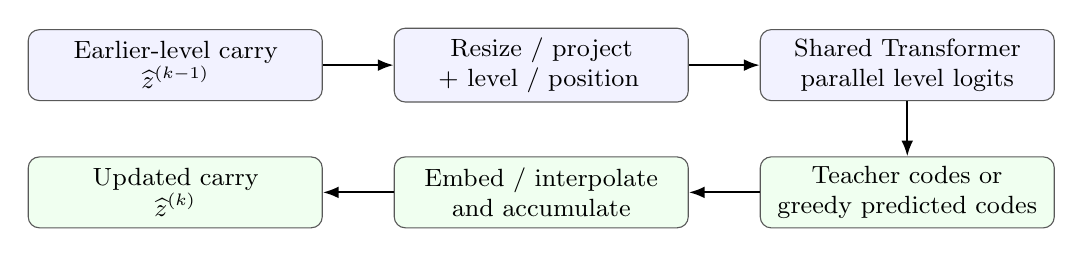
\begin{tikzpicture}[
  box/.style={draw=black!65,rounded corners,align=center,
    minimum height=9mm,text width=35mm,font=\small},
  flow/.style={-{Latex[length=2mm]},thick},node distance=7mm and 9mm]
  \node[box,fill=blue!5] (carry) {Earlier-level carry\\$\widehat z^{(k-1)}$};
  \node[box,fill=blue!5,right=of carry] (context) {Resize / project\\+ level / position};
  \node[box,fill=blue!5,right=of context] (prior) {Shared Transformer\\parallel level logits};
  \node[box,fill=green!6,below=of prior] (codes) {Teacher codes or\\greedy predicted codes};
  \node[box,fill=green!6,left=of codes] (add) {Embed / interpolate\\and accumulate};
  \node[box,fill=green!6,left=of add] (next) {Updated carry\\$\widehat z^{(k)}$};
  \draw[flow] (carry)--(context);
  \draw[flow] (context)--(prior);
  \draw[flow] (prior)--(codes);
  \draw[flow] (codes)--(add);
  \draw[flow] (add)--(next);
\end{tikzpicture}
\caption{One level of the scanned prior. Current-level teacher codes are
introduced after the logits are computed. The updated carry is the input to
the next level. Fallback features enter the final decoder separately.}
\label{fig:prior}
\end{figure}

\section{Training Objective and Gradient Boundaries}
The implemented objective is
\begin{equation}
 \mathcal{L}=\mathcal{L}_{\mathrm{recon}}
 +\beta\mathcal{L}_{\mathrm{commit}}
 +\lambda_H\mathcal{L}_{H}
 +\lambda_C\mathcal{L}_{\mathrm{concept}}
 +\lambda_{\mathrm{prior}}\mathcal{L}_{\mathrm{prior}}.
 \label{eq:total}
\end{equation}
Default coefficients are \(\beta=0.25\), \(\lambda_H=0.01\),
\(\lambda_C=0\), and \(\lambda_{\mathrm{prior}}=1\). Coefficients are
configuration choices, not experimentally optimized settings.

\subsection{Reconstruction and commitment}
Let \(p_\psi\) be the token decoder distribution. Reconstruction includes every
valid token, including slots using byte features:
\begin{equation}
 \mathcal{L}_{\mathrm{recon}}=
 -\frac{\sum_{b,t}m_{bt}\log p_\psi(x_{bt}\mid\widetilde z)}
 {\safe{\sum_{b,t}m_{bt}}}.
\end{equation}
The fallback-selected representation \(\widetilde z\) is defined in
Section~\ref{sec:fallback}. Commitment is a mean over all valid scalar
residual components, rather than an unweighted mean of per-level means:
\begin{equation}
 \mathcal{L}_{\mathrm{commit}}=
 \frac{\sum_{k,b,t}a_{kbt}\|u_{kbt}-\sg[q_{kbt}]\|_2^2}
 {\safe{D\sum_{k,b,t}a_{kbt}}}.
\end{equation}

\subsection{Differentiable marginal entropy}
An entropy computed only from hard argmin counts has zero encoder derivative
almost everywhere. The implementation therefore uses soft assignment masses
for the regularizer, while retaining hard assignments for EMA and diagnostics:
\begin{align}
 \pi_{kbtv}&=\operatorname{softmax}_{v}
  \left(-\|u_{kbt}-E_{kv}\|_2^2/\tau\right),\\
 \bar c_{kv}&=\sum_{b,t}a_{kbt}\pi_{kbtv},\qquad
 p_{kv}=\frac{\bar c_{kv}}{\max(\sum_{v'}\bar c_{kv'},10^{-8})},\\
 \mathcal{L}_H&=\sum_{k=1}^{K}w_k\sum_{v=0}^{V-1}
                  p_{kv}\log(p_{kv}+\epsilon_H).
\end{align}
The default temperature is \(\tau=1\), \(\epsilon_H=10^{-5}\), and
\(w_k=K-k+1\). Empty levels
contribute zero. This is a smoothed, soft-assignment estimate of negative
marginal entropy; it need not equal the entropy of hard codes. Optimizing it
can increase uncertainty without increasing semantic usefulness. Experiments
must report hard code usage, reconstruction, and prior prediction jointly.

\subsection{Optional concept consistency}
The coarse feature is the first level's code vectors interpolated onto the
common grid. A learned dense projection \(P\) maps the completed
straight-through representation into the same feature dimension. Over the
intersection \(\mathcal{M}\) of valid coarse and learned-path positions,
\begin{equation}
 \mathcal{L}_{\mathrm{concept}}=
 \frac{\sum_{(b,t)\in\mathcal M}
  \left[1-\operatorname{cos}_{\delta}
   \left(\mathcal{A}_{U_1}(q_1,a_1)_{bt},P(z_{\mathrm{ST}})_{bt}\right)\right]}
 {\safe{|\mathcal M|}}.
\end{equation}
The implementation stabilizes each feature norm by
\(\sqrt{\|g\|^2+10^{-8}}\). When \(\mathcal M\) is empty the loss is zero.
The coarse hard-code path is non-differentiable; gradients train the projection
and can reach the encoder through the fine straight-through representation.
Cosine agreement is an auxiliary hypothesis, not a measured semantic property.

\subsection{Prior loss and joint optimization}
The prior is trained against aligned current-level code labels:
\begin{equation}
 \mathcal{L}_{\mathrm{prior}}=
 -\frac{\sum_{k,b,t}a_{kbt}
    \log p_\theta(i_{kbt}\mid\widehat z^{(k-1)},k,\mathcal G)}
 {\safe{\sum_{k,b,t}a_{kbt}}}.
\end{equation}
``Next'' refers to the next hierarchy level, not a one-position shift within
that level. A separate shifted token cross-entropy helper exists for an
optional token-causal extension; it is not the NCM prior objective.

One optimizer state holds encoder, decoder, projection, and prior parameters.
However, the hard indices and prior codebook gathers are stop-gradient values.
Thus prior CE trains the generator, not the encoder through code identities.
The codec still changes through reconstruction and auxiliary terms, so the
prior sees moving targets in joint training. A frozen-tokenizer prior phase
is an important future controlled comparison, not a completed training result.

\section{Runtime Phases and Byte Routing}
\subsection{Phase-dependent EMA eligibility}
Let \(\phi\) be a scalar runtime integer. Level \(k\), using one-based indexing,
is eligible for EMA if
\begin{equation}
 e_k=\Ind[\phi=0\ \lor\ k>K-2]\,
     \Ind\!\left[\sum_v c_{kv}>0\right].
\end{equation}
If \(e_k=0\), all three tensors \(E_k,C_k,S_k\) retain their old values.
For \(K\leq2\), all levels remain eligible. The final phase freezes coarse
\emph{codebook state}, not encoder or decoder parameters.

During joint-phase training, a Bernoulli selector with configured probability
\(p_d\) chooses whether to sample a per-example prefix cutoff uniformly from
\(\{1,\ldots,K\}\); otherwise all levels are retained. The mask enforces the
cutoff without changing array sizes. For \(\phi\ne0\), the retained depth is
always \(K\). The scalar predicate changes values inside the executable rather
than changing a static Python argument. If the finest level is dropped, the
prior still needs the original learned-path source mask; it must not infer
that mask from the dropped level alone.

\subsection{Fixed-shape fallback representation}
\label{sec:fallback}
Let \(b_{bt}\in\{0,\ldots,255\}\) be a byte ID supplied by the data producer
and \(F\in\R^{256\times D}\) its embedding table. The decoder input is
\begin{equation}
 \widetilde z_{bt}=m_{bt}\left[
    f_{bt}F_{b_{bt}}+(1-f_{bt})z_{\mathrm{ST},bt}\right].
\end{equation}
This selection occurs in the compiled graph. Fallback slots are excluded from
the learned encoder inputs, quantizer assignments, and EMA statistics; they
remain valid reconstruction targets.

The interface requires the input pipeline to expand unsuitable UTF-8 regions
into aligned byte slots before bucketing and to assign compatible decoder
labels. Arbitrary token vocabulary IDs do not determine those bytes by
themselves. Exact literal recovery requires retaining the byte IDs and masks
in the external representation; an embedding followed by a neural decoder is
not inherently lossless. A mixed token/byte serialization format, UTF-8 assembly,
and a policy for selecting unsuitable regions remain unimplemented.

\section{Functional Execution and SPMD Placement}
The train state is a pytree containing neural parameters \(\Theta\), optimizer
state \(\Omega\), codebook state \((E,C,S)\), and a step counter. The transition
has the form
\begin{equation}
 (\Theta',\Omega',E',C',S',t';\mathcal{D})
 =\operatorname{Step}(\Theta,\Omega,E,C,S,t;\mathcal B,\phi,\xi),
\end{equation}
where \(\xi\) is a random key and \(\mathcal D\) contains diagnostics.
Targets and gradients are computed from the old state, the optimizer updates
neural parameters, and EMA updates the explicit codebooks once. An all-padding
global batch preserves optimizer state, parameters, EMA state, and the step
counter. It is a semantic skip; this branch does not guarantee that all
otherwise-computed arithmetic is avoided by the compiled executable.

Quantization uses \code{jax.lax.scan}. The prior uses a lifted Flax scan that
broadcasts parameters and splits dropout keys~\citep{flaxscan}.
The train function has explicit input and output \code{NamedSharding}
contracts~\citep{jaxsharding}. The mesh axes are \code{dp}, for data
parallelism, and \code{fsdp}, for parameter partitioning.

\begin{table}[t]
\centering\small
\caption{Implemented placement policy. \(P\) denotes a JAX partition spec;
matrix/tensor axes are chosen by a deterministic divisibility heuristic.}
\label{tab:placement}
\begin{tabularx}{\linewidth}{@{}lY@{}}
\toprule
State or input & Placement\\
\midrule
Input batch, shape \([B,L]\) & \(P(\code{dp},\mathrm{None})\); global B is divisible by mesh dp size\\
Matrix/tensor parameter & Largest divisible axis sharded over \code{fsdp}; replicated over \code{dp}\\
Biases and norm scales & Replicated\\
Optimizer moments & Same shape-based placement rule as corresponding parameter leaves\\
Optimizer counters & Replicated\\
Codebooks \(E,C,S\) & Replicated over both mesh axes\\
Phase, random key, diagnostics & Replicated\\
\bottomrule
\end{tabularx}
\end{table}

\subsection{Reduce sufficient statistics exactly once}
The end-to-end step consumes \emph{global arrays}. A sum over the global batch
dimension has global semantics; XLA supplies the required communication for its
sharded execution. That path does not introduce an explicit axis-named
\code{psum}. In contrast, a local-array function under a bound manual mapping
needs its local statistics summed over the bound data axis~\citep{jaxmanual}:
\begin{equation}
 c_{kv}^{\mathrm{global}}=\sum_{d\in\mathrm{dp}}c_{kv}^{(d)},\qquad
 s_{kv}^{\mathrm{global}}=\sum_{d\in\mathrm{dp}}s_{kv}^{(d)}.
\end{equation}
The low-level quantizer and EMA functions expose an optional \code{axis_name}
for this case. If the quantizer has already reduced its outputs, EMA must not
reduce them again. A named mesh alone does not bind a collective axis inside
an ordinary global-array JIT function.

Mask-aware means similarly reduce numerators and denominators, rather than
averaging means of unequally padded shards. All replicas then apply the same
EMA equations to the same global statistics. Codebooks are not sharded along
\(V\); distributed nearest-neighbor lookup would require additional design.

\subsection{Multi-host boundary and Rust tooling}
The repository includes a helper to construct global batches from
process-local data. It requires distributed initialization before mesh creation
and coordinated calls across hosts. The example initializes a complete small
host state; scalable checkpoint restoration and multi-host initialization have
not been validated.

A proposed Rust layer would ingest corpora, expand fallback bytes, form length
buckets, validate IDs/masks, and produce shard files and metadata. It could also
coordinate runs and aggregate evaluation outputs. The neural forward passes,
gradients, optimizer, EMA, and collectives remain in JAX/XLA. This separation
defines an integration boundary; it is not a claim that a Rust pipeline has
already been implemented or benchmarked.

\section{Complexity and Potential Bottlenecks}
\label{sec:complexity}
The padded level storage supports one scan body shape, at a cost. Dense
nearest-neighbor distances require \(O(KBLVD)\) arithmetic; retained prior
logits use \(O(KBLV)\) elements. The implementation also constructs dense
resampling matrices with \(O(KL^2)\) elements, and its dense alignment
contractions can require \(O(KBL^2D)\) work. Masks enforce correctness but do
not by themselves eliminate these operations.

For \(J\) dense-attention Transformer blocks with hidden width \(H\) and
fixed feed-forward expansion, padded attention/MLP work is approximately
\begin{equation}
 O\!\left(KJB(L^2H+LH^2)+KBLHV\right).
\end{equation}
This is an operation-count model of the source layout, not a measurement of
the compiler's memory schedule or realized device throughput. Implementing
true per-level lengths could replace the repeated \(L\) terms with sums over
\(n_k\), but would change the compilation organization.

Two simple useful-position fractions are
\begin{equation}
 \eta_{\mathrm{levels}}=\frac{\sum_k n_k}{KL},\qquad
 \eta_{\mathrm{attention}}=\frac{\sum_k n_k^2}{KL^2}.
\end{equation}
For the example schedule \((2,4,8)\), these are approximately \(0.583\) and
\(0.438\), respectively, before content padding. They describe layout
utilization, not measured speedups. Replicated codebooks cost \(O(KVD)\) memory
per device; global sufficient-statistic aggregation communicates arrays of
sizes \([K,V]\) and \([K,V,D]\). Parameter sharding can introduce additional
communication. Reducing sequential prediction decisions to \(K\) does not
imply a corresponding wall-clock improvement over token-autoregressive models.

\section{Software Validation}
\label{sec:validation}
The local validation environment was macOS 26.6.2 on arm64, Python 3.12.16,
JAX/jaxlib 0.10.2, Flax 0.12.8, Optax 0.2.8~\citep{optax}, and NumPy 2.5.4. Computation used
the CPU backend and float32 arithmetic. The full test suite was rerun for this
manuscript and reported \textbf{11 passed}. Test duration is deliberately not
used as an algorithmic benchmark.

\begin{table}[t]
\centering\small
\caption{Observed software validation. Counts are pytest test functions;
each function contains multiple assertions. Virtual devices are CPU devices,
not TPU chips.}
\label{tab:tests}
\begin{tabularx}{\linewidth}{@{}lclY@{}}
\toprule
Test module & Count & Result & Main checked properties\\
\midrule
\code{test_rvq.py} & 4 & Pass & Nearest neighbors, residual sums, EMA equations,
freezing, padding, gradients, and dropout phases\\
\code{test_losses.py} & 3 & Pass & Empty masks, valid adjacent-token CE,
entropy gradients, cosine loss, and exact-match denominators\\
\code{test_model.py} & 3 & Pass & Label isolation, byte routing, decoder reuse,
compiled optimizer updates, and all-padding state preservation\\
\code{test_spmd.py} & 1 & Pass & Full training-state comparison on a virtual
\(2\times2\) mesh; explicit manual reductions\\
\bottomrule
\end{tabularx}
\end{table}

\subsection{Distributed comparison protocol}
A fresh interpreter exposes four virtual CPU devices using the setting
\begin{lstlisting}[language=bash]
XLA_FLAGS=--xla_force_host_platform_device_count=4
\end{lstlisting}
The integrated test uses
\(B=4\), \(L=4\), \((n_1,n_2,n_3)=(1,2,4)\), \(D=4\), \(V=4\),
token vocabulary \(W=16\), and a one-block prior with width 8 and two heads.
Its four examples contain 4, 3, 1, and 0 valid positions. These unequal
counts exercise global normalization under padding.

An unsharded global-array step and a \(2\times2\)
\code{dp}/\code{fsdp} step start from the same initialized state and random
keys. Every returned parameter, optimizer leaf, EMA leaf, step count, and
metric is compared with absolute and relative tolerance \(3\times10^{-5}\).
The test separately checks that all codebook leaves replicate and that at
least one parameter and optimizer leaf is actually sharded. The comparison
uses Adam with learning rate \(10^{-3}\) and \(\epsilon_{\mathrm{Adam}}=10^{-5}\)
to avoid amplifying roundoff in near-zero gradients. It does not assert
bitwise equivalence between reduction orders.

Additional local-array \code{pmap} checks sum artificial EMA statistics and
compare them against a direct global update. They also compare quantizer
counts, sums, soft counts, and commitment numerators/denominators across the
local/global paths with absolute tolerance \(10^{-6}\) and NumPy's default
relative tolerance. This manual path validates sufficient-statistic reduction,
not a complete independently implemented local-array training loop.

\subsection{Synthetic training execution}
The example executes three AdamW steps on a fixed synthetic batch with
\(B=2\), \(L=8\), \((n_1,n_2,n_3)=(2,4,8)\), \(D=16\), \(V=16\),
and \(W=256\). The prior uses two blocks, width 32, and four heads; concept
loss weight is 0.1. The final step switches to the final-two-level phase.
The example completes with finite reported objectives. It is an execution
check with a reused toy batch, not a corpus experiment, convergence study,
or held-out generalization result.

\section{Research Evaluation Plan}
\label{sec:plan}
The central hypothesis is that a hierarchy with explicitly controlled shapes
and placement can offer useful generation quality at favorable measured
accelerator cost. This hypothesis remains open. The following experiments
would separate representation quality, prediction quality, and systems behavior.

\paragraph{Tokenizer study.}
Fix a corpus, token vocabulary, byte-expansion protocol, and held-out split
before tuning. Compare a single-grid RVQ against multiple level schedules at
matched code capacity and parameter budget. Report token reconstruction CE,
token and sequence exact match, per-level usage/perplexity, actual serialized
bits including fallback and metadata, and padding overhead. Nominal code
capacity \(\sum_k n_k\log_2 V\) is not an achieved entropy-coded file size.

\paragraph{Prior study.}
Evaluate both teacher-forced code loss and free-running generation. Compare
shared versus independent level parameters, joint versus frozen-tokenizer
training, and clean versus perturbed earlier-level conditioning. Fix decoding
rules, output lengths, and seeds. An incorrect early prediction can affect all
later contexts, so per-level teacher-forced accuracy alone is insufficient.

\paragraph{Objective and phase ablations.}
Sweep \(\lambda_H\), \(\lambda_C\), temperature, entropy weights, dropout
probability, and phase duration, including zero-regularization controls.
Measure whether marginal diversity improvements survive in hard assignments
and decoded text. Compare codebook freezing with continued joint EMA and
measure encoder drift while coarse codebooks are fixed.

\paragraph{TPU systems study.}
Record TPU generation, host count, mesh dimensions, runtime versions,
precision, batch sizes, and all sequence shapes. Report compilation time
separately from synchronized steady-state throughput and latency; include
peak memory, collective costs, useful-token fractions, and checkpoint/input
overheads. Compare the padded scan against per-level static executables and
more efficient resampling/distance kernels. Sweep \code{dp}/\code{fsdp} meshes
and compare float32 with appropriate mixed-precision alternatives.

\paragraph{Matched end-to-end baselines.}
Compare against token-autoregressive Transformers, diffusion language models,
and the original NCM implementation under matched datasets, model capacities,
training budgets, and generation protocols. Report quality--cost curves rather
than a single speed ratio. Use multiple independent seeds where feasible and
report uncertainty and failures. No target threshold, including a requested
99.5\% token exact-match rate, is an achieved result for this repository.

\section{Limitations and Research Integrity}
\label{sec:limitations}
The current evidence supports a small tested reference implementation. It
does not establish TPU execution, multi-host reliability, useful learned
concepts, or competitive language modeling. CPU virtual devices exercise
sharding semantics but cannot stand in for TPU interconnects or memory limits.

The text codec is deliberately small and local. The prior has no user-prompt
cross-attention interface, learned length prediction, or stochastic sampling
policy in the evaluated code path. Its default first-level predictions are
unconditional on text content for fixed geometry. The joint interface also
does not automatically provide the staged training used by the original NCM
work. These are concrete boundaries for future extensions.

The dense resampling and common-length attention layout may become expensive
well before a useful language-model scale. There is no vocabulary-sharded
codebook lookup, dead-code recovery, fault-tolerant checkpoint lifecycle, or
corpus ingestion implementation. Byte routing is present, but the complete
mixed-symbol codec and fallback selection policy remain external. No Rust
performance or functionality is reported.

This paper credits the underlying NCM method to its original authors and
describes Fabian Balensiefer's project as an independent systems adaptation.
No text-generation benchmark, performance advantage, or novel semantic
capability is inferred from passing tests. The public repository citation and
source hashes provide provenance for this manuscript. The project URL is a
mutable development location; an archived release with a persistent identifier
would further improve long-term reproducibility.

\section{Conclusion}
The repository makes a multiscale NCM-style computation explicit as a
functional JAX/Flax program. Its core properties are mask-aware quantization,
EMA state returned from training steps, earlier-level-only prior conditioning,
runtime phase predicates, and declared distributed array placement. Eleven
passing CPU tests provide evidence for these behaviors, including a virtual
four-device state comparison. The next research step is a controlled training
and TPU evaluation program that measures representation utility and execution
cost while completing the surrounding data and byte-stream contracts.

\appendix
\section{Repository Map and Reproduction}
\label{app:repro}
The package version is 0.1.0. The companion
\code{source_manifest.sha256} records SHA-256 hashes of the source, tests,
example, package configuration, and repository README inspected for this
paper. It identifies the implementation snapshot independently of the current
head of the public repository:
\begin{center}
\url{https://github.com/fbalensiefer/Next-Concept-Modeling-for-TPU}
\end{center}

\begin{table}[h]
\centering\small
\caption{Repository components relevant to the manuscript. Paths are relative
to the repository root.}
\begin{tabularx}{\linewidth}{@{}lY@{}}
\toprule
Path & Responsibility\\
\midrule
\code{src/ncm/config.py} & Immutable shape, Transformer, and loss configuration\\
\code{src/ncm/grids.py} & Area-pooling and interpolation matrices; mask normalization\\
\code{src/ncm/rvq.py} & Quantizer scan, sufficient statistics, explicit EMA\\
\code{src/ncm/tokenizer.py} & Token codec, byte embedding selection, separate decoder API\\
\code{src/ncm/generator.py} & Shared Transformer level scan and greedy generation\\
\code{src/ncm/losses.py} & Normalized reconstruction, commitment, entropy, concept, and CE terms\\
\code{src/ncm/training.py} & Joint model, complete training state, optimizer/EMA step\\
\code{src/ncm/sharding.py} & Mesh, placement, process-local input helper, compiled contract\\
\code{src/ncm/metrics.py} & Exact match, hard usage, and perplexity utilities\\
\code{tests/} & Unit, integration, and virtual multi-device checks\\
\code{examples/train.py} & Three-step synthetic execution example\\
\bottomrule
\end{tabularx}
\end{table}

A fresh CPU environment can run:
\begin{lstlisting}[language=bash]
python3.12 -m venv .venv
source .venv/bin/activate
pip install -e '.[test]'
pytest -q
python examples/train.py
\end{lstlisting}
The declared dependency ranges permit versions other than the tested stack;
pin the versions listed in Section~\ref{sec:validation} for closer
reproduction. The multi-device pytest entry launches its own CPU subprocess.
For manuscript compilation, this single file uses standard LaTeX packages
and embeds the bibliography; no external figure or bibliography file is needed.

\section{Global Training Transition}
\begin{lstlisting}[language=Python]
def step(state, batch, phase, key):
    # Global arrays: no explicit data-axis psum here.
    (loss, (metrics, rvq)), grads = value_and_grad(
        objective, has_aux=True)(state.params)
    updates, opt_state = optimizer.update(
        grads, state.opt_state, state.params)
    params = apply_updates(state.params, updates)
    codebooks = ema_update(
        state.codebooks, rvq.counts, rvq.sums,
        config, phase=phase)  # statistics already global
    candidate = TrainState(
        params, opt_state, codebooks, state.step + 1)
    return cond(any(batch.mask), candidate, state), metrics
\end{lstlisting}
This schematic omits the objective closure and JAX call syntax details;
\code{make_train_step} is the executable implementation. State is returned
explicitly and can be supplied to the next compiled call. A scalable
checkpointing layer must additionally retain configuration, random-key
progression, and data-iterator position to reproduce an interrupted run.

\begingroup
\raggedright
\begin{thebibliography}{99}

\bibitem[Kumbong et~al.(2026)]{kumbong2026ncm}
Hermann Kumbong, Ishan S. Khare, Iddah Mlauzi, Andrew Woen, Charles Ding,
E. Kelly Buchanan, Simran Arora, Azalia Mirhoseini, and Christopher R\'e.
\newblock Next-Concept Modeling: Fast, Parallel Coarse-to-Fine Text Generation.
\newblock \emph{arXiv preprint arXiv:2610.14162}, 2026.
\newblock \url{https://arxiv.org/abs/2610.14162}.

\bibitem[van~den Oord et~al.(2017)]{oord2017vqvae}
Aaron van~den Oord, Oriol Vinyals, and Koray Kavukcuoglu.
\newblock Neural Discrete Representation Learning.
\newblock \emph{Advances in Neural Information Processing Systems}, 30, 2017.
\newblock \url{https://arxiv.org/abs/1711.00937}.

\bibitem[Zeghidour et~al.(2021)]{zeghidour2021soundstream}
Neil Zeghidour, Alejandro Luebs, Ahmed Omran, Jan Skoglund, and Marco
Tagliasacchi.
\newblock SoundStream: An End-to-End Neural Audio Codec.
\newblock \emph{arXiv preprint arXiv:2107.03312}, 2021.
\newblock \url{https://arxiv.org/abs/2107.03312}.

\bibitem[Vaswani et~al.(2017)]{vaswani2017attention}
Ashish Vaswani, Noam Shazeer, Niki Parmar, Jakob Uszkoreit, Llion Jones,
Aidan N. Gomez, \L{}ukasz Kaiser, and Illia Polosukhin.
\newblock Attention Is All You Need.
\newblock \emph{Advances in Neural Information Processing Systems}, 30, 2017.
\newblock \url{https://arxiv.org/abs/1706.03762}.

\bibitem[Lepikhin et~al.(2020)]{lepikhin2020gshard}
Dmitry Lepikhin, HyoukJoong Lee, Yuanzhong Xu, Dehao Chen, Orhan Firat,
Yanping Huang, Maxim Krikun, Noam Shazeer, and Zhifeng Chen.
\newblock GShard: Scaling Giant Models with Conditional Computation and
Automatic Sharding.
\newblock \emph{arXiv preprint arXiv:2006.16668}, 2020.
\newblock \url{https://arxiv.org/abs/2006.16668}.

\bibitem[Bradbury et~al.(2018)]{jax}
James Bradbury, Roy Frostig, Peter Hawkins, Matthew James Johnson,
Yash Katariya, Chris Leary, Dougal Maclaurin, George Necula, Adam Paszke,
Jake VanderPlas, Skye Wanderman-Milne, and Qiao Zhang.
\newblock JAX: Composable transformations of Python+NumPy programs.
\newblock Software, 2018; version 0.10.2 used in this work.
\newblock \url{https://github.com/jax-ml/jax}.

\bibitem[Heek et~al.(2020)]{flax}
Jonathan Heek, Anselm Levskaya, Avital Oliver, Marvin Ritter,
Bertrand Rondepierre, Andreas Steiner, and Marc van~Zee.
\newblock Flax: A neural network library and ecosystem for JAX.
\newblock Software, 2020; version 0.12.8, Linen API, used in this work.
\newblock \url{https://github.com/google/flax}.

\bibitem[OpenXLA Project(2026)]{xla}
OpenXLA Project.
\newblock XLA documentation.
\newblock \url{https://openxla.org/xla}. Accessed November 11, 2026.

\bibitem[Optax Developers(2026)]{optax}
Optax Developers.
\newblock Optax: A gradient processing and optimization library for JAX.
\newblock Software, version 0.2.8 used in this work.
\newblock \url{https://github.com/google-deepmind/optax}.
Accessed November 11, 2026.

\bibitem[JAX Authors(2026a)]{jaxsharding}
JAX Authors.
\newblock \code{jax.sharding} module: Mesh, NamedSharding, and PartitionSpec.
\newblock \url{https://docs.jax.dev/en/latest/jax.sharding.html}.
Accessed November 11, 2026.

\bibitem[JAX Authors(2026b)]{jaxmanual}
JAX Authors.
\newblock Manual parallelism with \code{shard_map}.
\newblock \url{https://docs.jax.dev/en/latest/201/shard-map.html}.
Accessed November 11, 2026.

\bibitem[Flax Authors(2026)]{flaxscan}
Flax Authors.
\newblock Linen transformations: \code{flax.linen.scan}.
\newblock \url{https://flax-linen.readthedocs.io/en/latest/api_reference/flax.linen/transformations.html}.
Accessed November 11, 2026.

\bibitem[Balensiefer(2026)]{localrepo}
Fabian Balensiefer.
\newblock Next-Concept Modeling for TPU.
\newblock Public software repository, package \code{tpu-ncm}, version 0.1.0,
snapshot of November 11, 2026.
\newblock \url{https://github.com/fbalensiefer/Next-Concept-Modeling-for-TPU}.
\newblock Source, tests, and example accompany this manuscript; snapshot hashes
are recorded in \code{paper/source_manifest.sha256}. Accessed November 11, 2026.

\end{thebibliography}
\endgroup
\end{document}
